\chapter{Thickness inference using thermal imaging} \label{Thickness inference using thermal imaging}
\minitoc

% A few considerations:
% 1) The mathematical notation should be changed accordingly to Yves's suggestion in the paper
% 2) Some Figure could be replaced or improved. For instance, the Figure 4.7 should be replaced as well as the 4.15.

% Notation
% n --> samples (i=1...n)
% K=20 --> number of critical points (k=1...K)
% X_i --> thermal video
% Y_i --> Thickness vector 
% x_{ik} --> 


\section{Introduction}

In the previous chapter, we showed the difficulty of inferring the weight of the tank given the process parameters as they are collected today. The possible explanations have been addressed in section \ref{Results and Discussions}. The weight is a quality indicator that summarises the information about the overall amount of material which composes the fuel tank. However, as we saw earlier, the weight does not guarantee the correct distribution of the material over the whole surface, as different thickness distributions may lead to the same weight. As a consequence, we decided to focus directly on thicknesses, which provide more accurate information about the distribution of the material over the surface. Of course, measuring the tank thicknesses using the only the available process parameters could be challenging as we have no information about the geometry of the tank. It is therefore necessary to collect new data that can provide us with spatial information.

In this chapter, we propose a new approach to perform a real-time, non-destructive quality control to measure thicknesses of blow-moulded parts. The proposed approach makes use of deep learning data-driven methods to leverage the thermal inertia of the manufactured plastic part, captured through thermal imaging, to infer the thicknesses of the part surface without any direct measurement. Compared to traditional quality inspection approaches, which aims to detect visual defects of manufactured products, our approach leverages thermal information to perform a non-visual quality control. The first experimental results on real industrial data are very promising and demonstrate that the proposed method could achieve satisfactory performance in industrial conditions.

\section{Weight and thicknesses}

Before digging into the details of the proposed approach, it is interesting to explore the relationship between the thickness values and the tank weight. In order to asses if there exist a measurable statistical relationship between the weight and the tank thickness a simple correlation analysis has been conducted. By taking advantage of 300 measured tanks, for which the weight, as well as the thickness of a limited number of critical points, the correlation between each thickness-weight pair is computed. Figure \ref{fig:thickness_points} shows the coordinates of the six points for which the thickness was measured. 
%
\begin{figure}
\centering
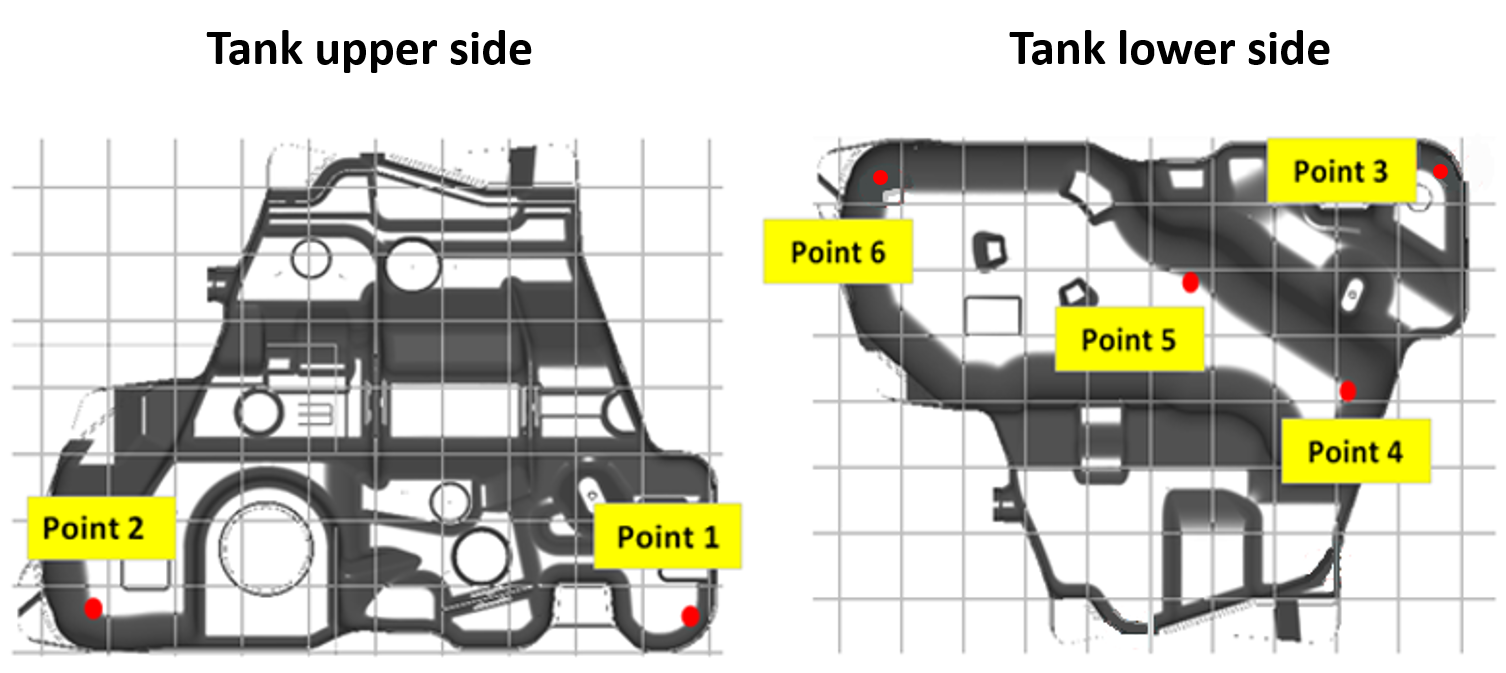
\includegraphics[scale=0.55]{images/chapter_4/Thickness_points.png}
\caption{Thickness points}
\label{fig:thickness_points}
\end{figure}
%
Figure \ref{fig:thicknesses_weight_scatter} shows the scatter plots drawn by plotting each thickness-weight pair, with one variable on each axis. For each plot, the regression line is drawn to visualise the trend. As visible in the Figure, there exist a minor correlation between some of the thickness points and the tank weight. The highest correlation, between the thickness at point 5 and the weight, is 0.40: there is a lot of dispersion within data, and a higher weight does not mean a higher thickness. This confirms our assumption that it is impossible to ensure the correct distribution of material over the surface of the tank by monitoring solely the weight. 
%
\begin{figure}
\centering
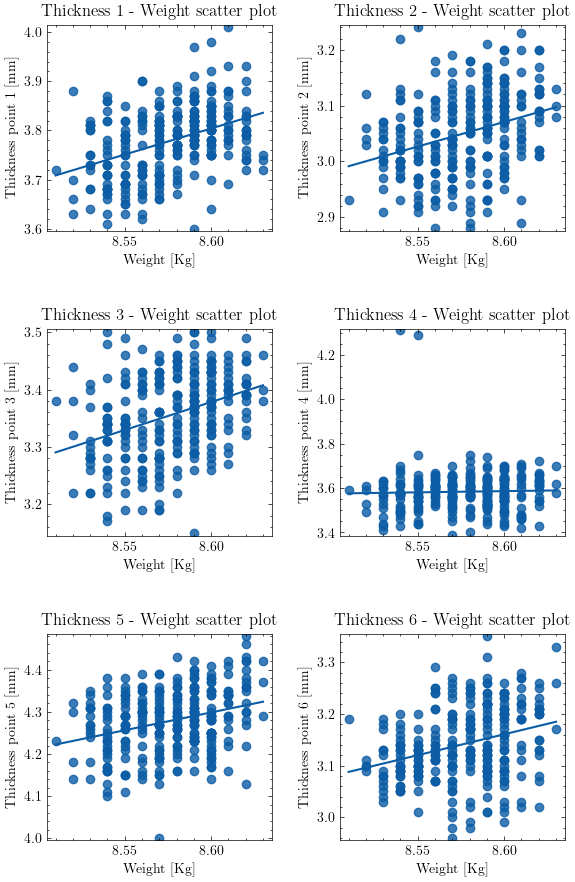
\includegraphics[scale=0.9]{images/chapter_4/thickness_weight.png}
\caption{Thicknesses - weight scatter plots}
\label{fig:thicknesses_weight_scatter}
\end{figure}
%
The weight and the sum of the 6 measured thicknesses are slightly more correlated (Figure \ref{fig:thickness_sum_weight_correlation}) as expected since the weight is proportional to the amount of material composing the fuel tank.
%
\begin{figure}
\centering
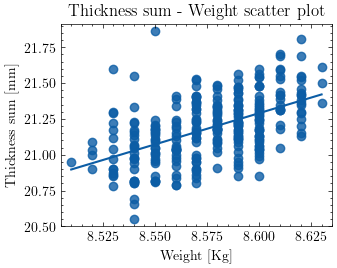
\includegraphics[scale=1]{images/chapter_4/thickness_sum_weight.png}
\caption{Thickness sum - Weight correlation}
\label{fig:thickness_sum_weight_correlation}
\end{figure}
%
Results presented in this section show that the weight of the tank is not sufficient to ensure the correct distribution of the material along the surface. In order to improve quality control and ensure that thicknesses meet customer specifications it is advisable to focus our research work directly towards the inference of thicknesses.

\section{Motivation} \label{Motivation}

Our work is motivated by the empirical observation of the cooling of blow-moulded parts in the first minutes after blowing. Areas of the parts have different cooling behaviours depending on their thickness. 

Areas with smaller thicknesses cool down faster than those with higher thicknesses. For the thicker zones, the surface temperature even starts to increase before decreasing (Figure~\ref{fig:temperature_cooling}).
%
\begin{figure}
\centering
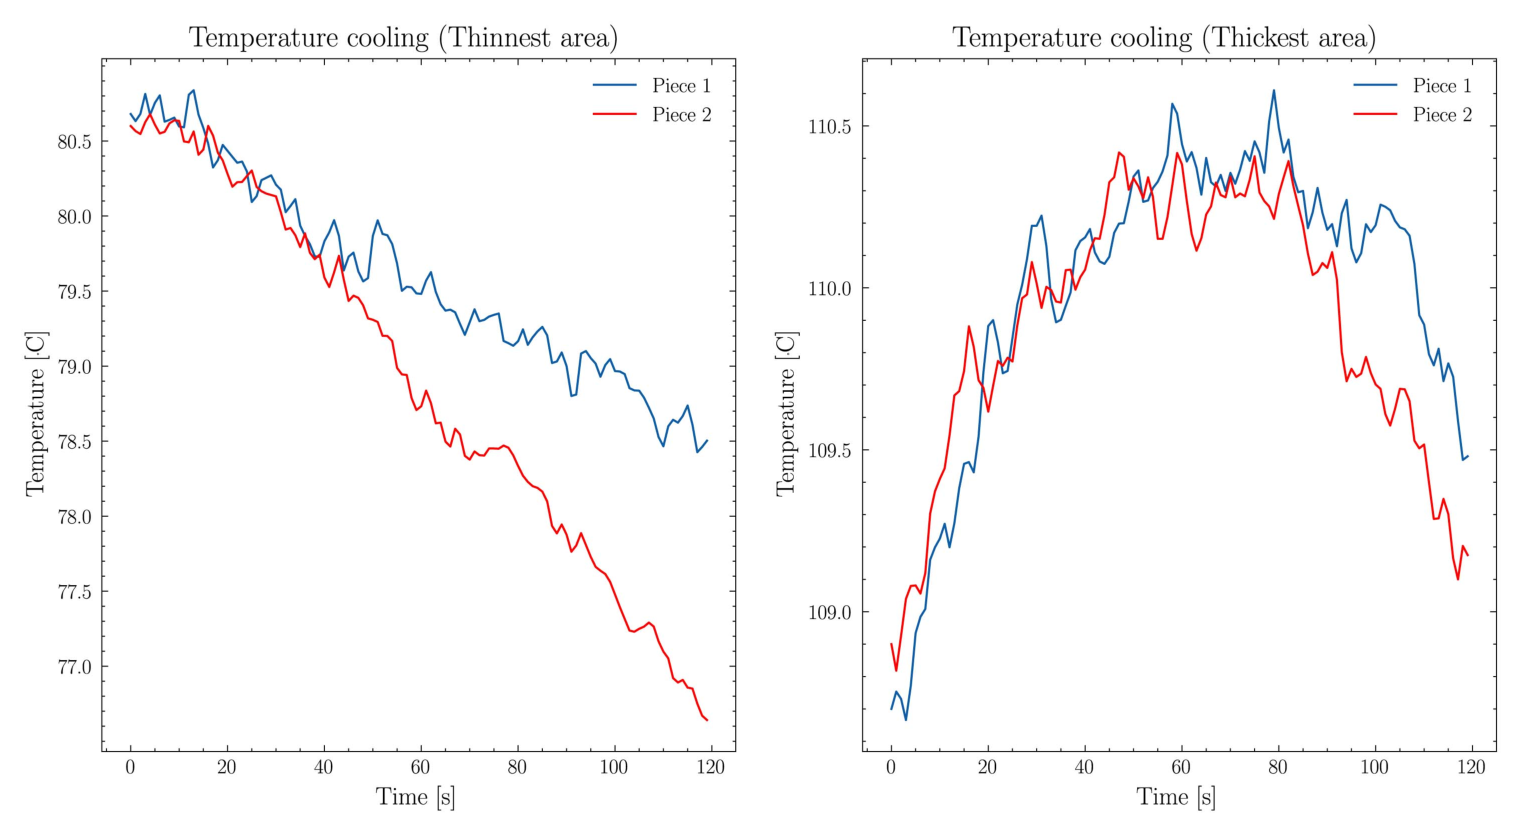
\includegraphics[scale=0.55]{images/chapter_4/cooling.eps}
\caption{Surface temperature cooling profiles at the thinnest (left) and thickest (right) areas of the blow-moulded part}
\label{fig:temperature_cooling}
\end{figure}
%
This phenomenon is due to the release of energy from the innermost plastic layer that has not be in direct contact with the mould surfaces.
As suggested by the literature presented in Section \ref{Background}, this surface temperature decay, easily measured by thermal imaging, could be leveraged to infer the thickness of the part.  
In particular, we make two assumptions:
\begin{itemize}
   \item The cooling conditions of the environment where the part is monitored are the same for all parts produced. Therefore, we consider that the variations of the temperature of the production area are negligible.
   \item The physical and chemical properties of the material are assumed to be constant over the entire surface of the part. In particular, the thermal and infrared transmittances of the material should be approximately constant.
\end{itemize}

Based on these assumptions, we designed two data-driven methods to model the relationship between the surface temperature variations of critical areas of the part and the corresponding thickness values. The first approach, by one-dimensional time series, exploits the cooling dynamics, one point of the part at a time, whereas the second method processes the part globally, taking into account unity of part (points belonging to the same part are processed simultaneously) and spatial information (points are positioned on the part surface).

\section{Proposed methods}

In this section, we present new approaches to predict the thickness of blow-moulded parts. We propose a non-intrusive real-time thickness inference exploiting the variations of surface temperatures over time on different areas of the blow-moulded part. 
Unlike traditional thickness quality control methods, our system is able to predict thickness values at critical points of the part within minutes, allowing real-time operation.

Three different approaches to model the temperature-thickness relationship are proposed:
%
\begin{itemize}
    \item \textit{Parametric temporal approach}: The Parametric temporal approach involves the use of a parametric function to approximate the pointwise temperature surface decay. The function parameters, retrieved through curve fitting, may then be used as input features for a machine learning regressor.
    \item \textit{Flexible temporal approach}: The flexible temporal approach, as the parametric temporal one, takes advantage of the pixel-wise temperature decay. Instead of compressing the information through the use of a parametric function, the flexible temporal approach leverages the ability of deep learning to extract meaningful features from raw signals.
    \item \textit{Spatio-Temporal approach}: The spatio-temporal approach leverages not only the temporal temperature information, but also the spatial one. Instead of extracting the temperature time series for each critical point of the blow-moulded parts we can design an \textit{end-to-end} deep learning architecture able to directly handle the input thermal video. In such a way, we should be able to take into account the tank unit intrinsic information which is completely lost in the previous approaches.
\end{itemize}
%
These three approaches are presented in more detail below.

\subsection{Parametric temporal approach} \label{Parametric Temporal approach}

The first approach consists of three phases: time series extraction, time series approximation by parametric curve fitting and thickness prediction using the parameters of the approximated temperature surface decay.

\paragraph{Time series extraction:} 

The time series extraction phase aims to process the input thermal video in order to retrieve the temperature time series of a limited number of critical points, for which the thickness value is known. These time series constitute the input data of our data-driven model. Given $K$ critical points of each part for which the thickness values are known, and given the thermal video $X_{i}$, we are interested in extracting the time series ${x}_{ik} = \left (X_{i}(\xi_{k}, \zeta_{k},1),\ldots,X_{i}(\xi_{k}, \zeta_{k},T) \right) \in \mathds{R}^{T}$ with $T$ time steps, where $(\xi_{k}, \zeta_{k}) \in \{1,\ldots,h\}\times\{1,\ldots,w\}$ indexes the pixel corresponding to key point $k \in \{1,\ldots,K\}$. For a set of $n$ input thermal videos, this first phase produces a dataset
\begin{equation}
    D = \left\{\{x_{ik},y_{ik}\}_{k=1}^K\right\}_{i=1}^n
\end{equation}
of $K \times n$ pairs $(x_{ik},y_{ik})$ where $x_{ik} \in \mathds{R}^{T}$ is the time series corresponding to key point $k$ in thermal video $i$ and $y_{ik} = Y_{i}(\xi_{k}, \zeta_{k}) \in \mathds{R}$ is the corresponding thickness value.


\paragraph{Time series approximation:}

In order to reduce the number of input features we approximate the surface-temperature decay time series by a parametric expansion,  to compress the temporal information into a limited number of new features, corresponding to the parameters of the function. Temperature-surface time series have a fairly simple shape (Figure \ref{fig:temperature_cooling}). The predominantly parabolic shape of the time series lends itself well to be approximated with simple functions, with few parameters. We compared the following three parametric models:
\begin{itemize}
    \item Power Law: $y=ax^b$,
    \item Polynomial (2nd degree): $y=ax^2+bx+c$,
    \item Logarithmic: $y=a+b\log(x)$.
\end{itemize}

In such a way, the different cooling behaviour, observable in different areas of the part could be expressed through a limited number of new parameters. Moreover, the functional approximation smooths the time signal, thereby filtering the measurement noise. The new features may be then used as the input data for a regression model.
Mathematically speaking, the time series approximation produces a new dataset,
%
\begin{equation*}
    D = \left\{\{z_{ik},y_{ik}\}_{k=1}^K\right\}_{i=1}^n
    \enspace,
\end{equation*}
%
composed of $K\times n$ pairs $(z_{ik},y_{ik})$ collection pairs where ${z}_{ik} \in \mathds{R}^{P}$ are the $P$ parameters obtained by fitting the parametric function to the time series $x_{ik}$.

\begin{sidewaysfigure}
\centering
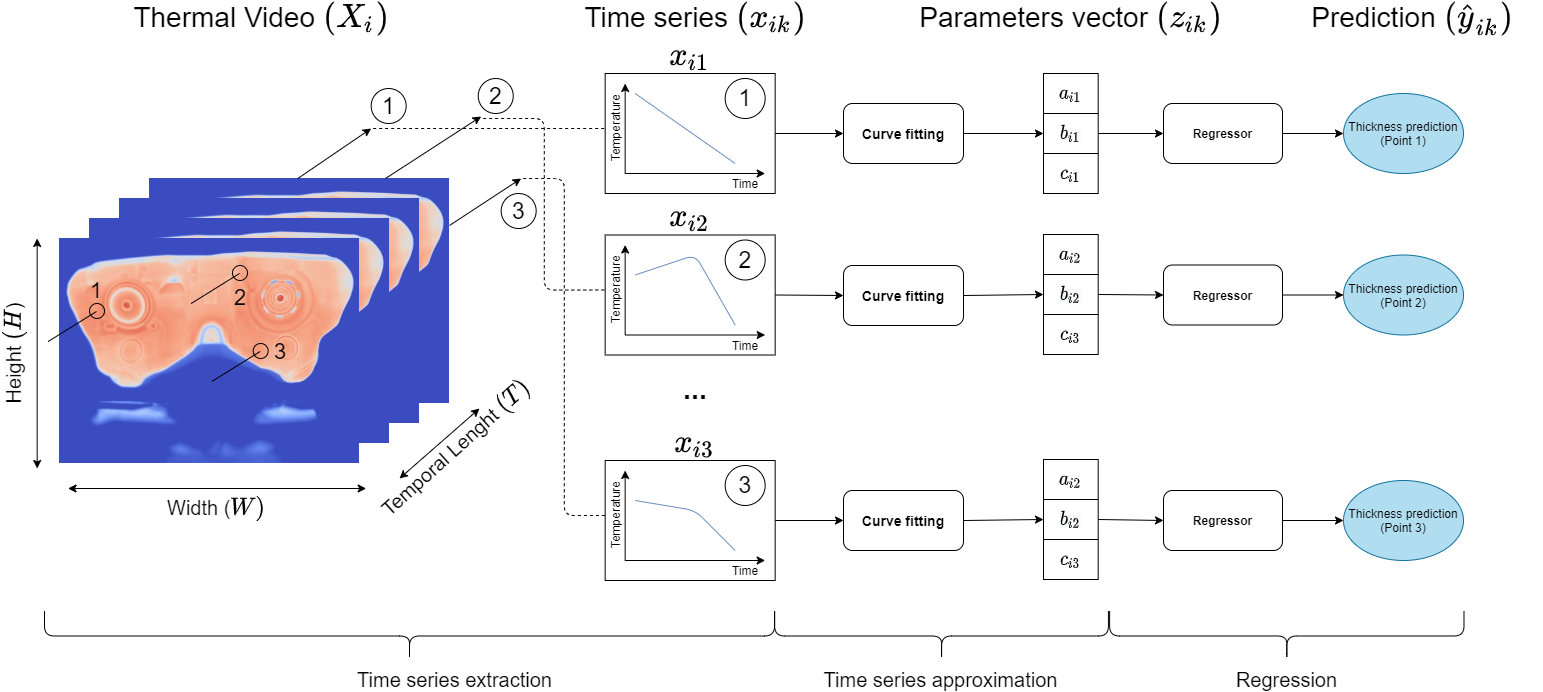
\includegraphics[scale=0.4]{images/chapter_4/Parametric_Temporal.png}
\caption{Parametric temporal approach}
\label{fig:parametric_temporal_approach}
\end{sidewaysfigure}

\paragraph{Time series regression:}
Any machine learning method can then be applied to predict the thickness value of a given key point based on the parameters computed by fitting the surface-temperature time series.  The role of the machine learning algorithm is to estimate a function $\hat{g}$ such that
\begin{equation}
    \hat{g} = \argmin_{g \in \mathcal{G}} \sum_{i=1}^n \sum_{k=1}^K (y_{ik} - g(z_{ik}))^2 \enspace.
\end{equation}


\subsection{Flexible temporal approach}

As illustrated in Figure \ref{fig:temporal_approach}, the proposed method consists of two phases: extraction of the time series and thickness value regression through a recurrent neural network (RNN). The time series extraction is carried out exactly in the same way as for the parametric temporal approach (see Section \ref{Parametric Temporal approach}).  

\begin{sidewaysfigure}
\centering
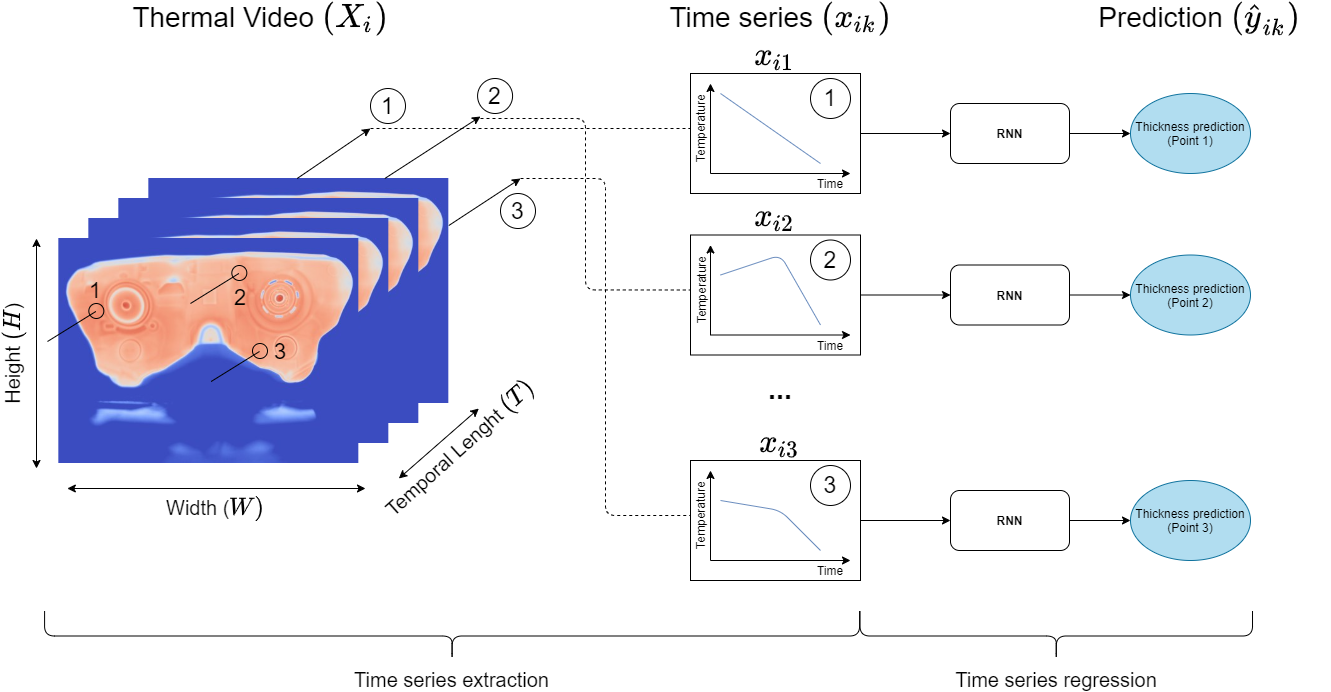
\includegraphics[scale=0.4]{images/chapter_4/Flexible_Temporal.png}
\caption{Flexible temporal approach}
\label{fig:temporal_approach}
\end{sidewaysfigure}

\paragraph{Time series regression:}

Given the extracted time series and the corresponding thickness values, our problem can be formulated as a supervised machine learning problem, more specifically, as a univariate time series regression problem. With univariate time series regression we mean the task of predicting the real number value of the dependent variable, the thickness, given a single dependent variable corresponding to a sequence of discrete-time data. Formally, we look for function $\hat{g}$ such that
\begin{equation}
    \hat{g} = \argmin_{g\in\mathcal{G}} \sum_{i=1}^n \sum_{k=1}^K (y_{ik} - g(x_{ik}))^2 \enspace.
\end{equation}
%
As our hypothesis is that temporal information plays a key role in thickness discrimination, we chose to use a recurrent neural network (see Section \ref{Recurrent Neural Network}) to model the dependency. 
%
\begin{figure}
\centering
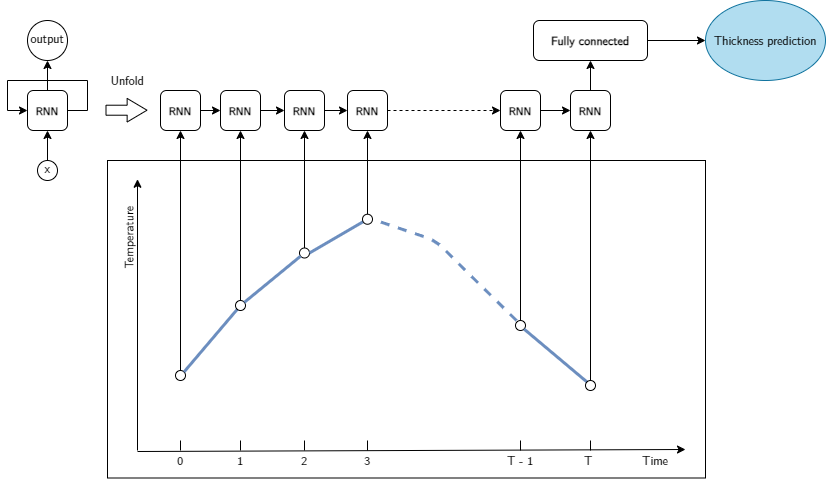
\includegraphics[scale=0.45]{images/chapter_4/rnn_model.png}
\caption{RNN-based model}
\label{fig:rnn_model}
\end{figure}
%
Inspired by the results achieved by RNNs in the domain of sequential data, we designed a simple RNN to address our problem (Figure \ref{fig:rnn_model}). The main idea behind our pipeline is to sequentially process the temperature at each time step $t$ by taking into account information from prior inputs to predict the current input and output. The last output computed by the RNN model is then passed through a fully connected layer to produce a scalar output aiming at approximating the thickness of the part area for which the time series has been extracted.

\subsection{Spatio-Temporal approach} \label{Spatio-temporal approach}

Compared to the previous approaches, the method proposed in this section aims to leverage not only the temporal temperature information, but also the intrinsic information of the tank unit. Instead of extracting the temperature time series for each critical point of the blow-moulded parts we design an \textit{end-to-end} deep learning architecture capable of directly processing thermal video as input data. In this setup, the dataset
\begin{equation}
    D = \{(X_{i}, Y_{i})\}_{i=1}^{n},
\end{equation}
is a collection of pairs $(X_{i}, Y_{i})$ where $X_{i} \in \mathds{R}^{h \times w \times T}$ is the input thermal video made of $T$ frames of height $h$ and width $w$, and $Y_{i} \in \mathds{R}^{h \times w}$ is the corresponding thickness image, that is, the 2D array of thicknesses on each of the input pixels. The role of the spatio-temporal approach is to estimate a function $\hat{g}$ such that
\begin{equation}
    \hat{g} = \argmin_{g\in\mathcal{G}} \sum_{i=1}^n \left( Y_{i} - g(X_{i})\right)^2 \enspace,
\end{equation}
or more precisely such that
\begin{equation}
    \hat{g} = \argmin_{g\in\mathcal{G}} \sum_{i=1}^n \sum_{k=1}^K \left( Y_{i}(\xi_{k}, \zeta_{k}) - g(X_{i}(\xi_{k}, \zeta_{k})\right)^2 \enspace,
\end{equation}
where $(\xi_{k}, \zeta_{k}) \in \{1,\ldots,h\}\times\{1,\ldots,w\}$ indexes the pixel corresponding to the key point $k$.

The work presented in this paragraph is inspired by the computer vision domain of \textit{semantic segmentation}, whose objective is to classify  the pixels of an image that belong to the same object class. Basically for an input image, semantic segmentation produces a segmentation mask which has the same spatial dimension of the input image where each pixel value correspond to the predicted class. As for other computer vision tasks, state-of-the-art results are obtained by convolutional neural networks (see Section \ref{Convolutional Neural Network}).
Here, instead of predicting a segmentation mask per image and per class, we propose to use a encoder-decoder architecture to learn thicknesses from a thermal video sequence. As before, thicknesses are only measured on the key points of the part. The end-to-end pipeline that infers the thicknesses of the key points from the thermal video sequence is depicted in Figure \ref{fig:spatio_temporal_architecture}.
%
\begin{sidewaysfigure}
\centering
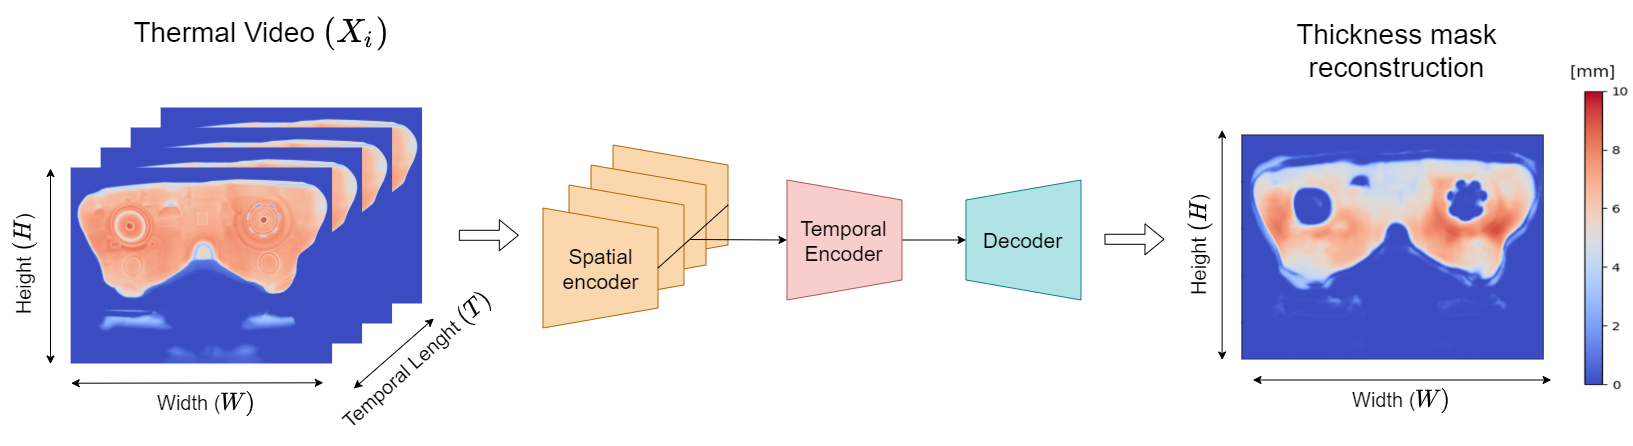
\includegraphics[scale=0.35]{images/chapter_4/Spatio-Temporal.png}
\caption{Spatio-Temporal architecture}
\label{fig:spatio_temporal_architecture}
\end{sidewaysfigure}
%
The proposed pipeline is largely inspired by the \textit{Unet} (see Section \ref{U-Net}), and consists of three main blocks: the spatial encoder, the temporal encoder and the spatial decoder. 

\begin{itemize}
    \item \textit{Spatial Encoder:} The spatial encoder is a CNN which aims to extract the spatial feature map for each frame of the video. 
    We use the encoder of a traditional encoder-decoder architecture. Compared to the original \textit{Unet} architecture, we replace the original contracting path proposed in the paper with a Residual Network (ResNet, see Section \ref{Residual Networks}). The ResNet architecture is composed of five main building blocks. Each block sequentially produces higher-level and lower-resolution features which will later be used by the decoder to predict thicknesses. The general input thermal video is a four-dimensional tensor of shape $(h, w, c, t)$ where $h$, $w$, $c$ and $t$ are respectively the height of the image, the width, the number of channels and the number of frames of the video sequence. The spatial encoder processes each frame $(h, w, c)$ of the input thermal video and returns a feature map of size $(h', w', c', t)$ where $h'<<h$, $w'<<w$ and $c'>>c$ and a set of intermediate feature maps.
    

    \item \textit{Temporal Encoder:} The temporal encoder aims to encode the temporal information of the spatial feature maps produced by the spatial encoder, which encodes each frame independently, without leveraging any kind of temporal information. In order to process the temporal information, we use a 3D convolutional layer with a kernel size of $(1\times1\times1)$, stacked right after the spatial encoder, which produces a linear projection of the stack of frame-wise feature maps. This projection acts as a dimensional reduction along the temporal axis. In such a way we are able to produce a new feature map which encodes both the spatial and the temporal information. Given the spatial feature map of size $(h', w', c', t)$, the temporal decoder compress the temporal dimension and produces a new \textit{spatio-temporal feature map} with size $(h', w', c', 1)$.  The same convolutional operation, with the same parameters, is applied to compress the temporal information of all the intermediate features maps produced by the spatial encoder.
    
    \item \textit{Decoder:} The decoder projects the discriminant spatio-temporal feature map back to the original input spatial dimension. In the same way as for the \textit{Unet} architecture, intermediate high-level low-resolution features from the encoder path are combined and reused with the upsampled output of each decoder block to help the model reconstructing the prediction mask. The decoder is composed on five decoder blocks and each decoder block applies an upsample operation using the nearest neighbour algorithm followed by two 2D convolutional layers with a kernel size of $3\times 3$, batch normalisation and \textit{ReLu} activation function. A final convolutional layer produces the thickness map from which the prediction of the thickness of the critical  points is extracted. Given the encoded pattern of size $(h', w', c', 1)$ the decoder projects the encoded pattern to the original spatial dimension producing a 1-channel map reconstruction $(h, w, 1)$. Given the pixel coordinates of the $n$ critical points, their corresponding thickness predictions can be easily retrieved.
\end{itemize}

Training such an architecture is more challenging compared to that of the flexible temporal approach because of the number of learnable parameters. Furthermore, we have two main shortcomings:

\begin{itemize}
    \item The size of the training sample is low compared to what is normally used to train this kind of network. For semantic segmentation tasks, a dataset of 1000 images is considered small and we could hardly have more than a few hundred input samples.
    \item The thickness ground-truth map is not known for all the points of the tanks. In the training phase, semantic segmentation requires the output mask of the input data. For our problem, we do not have access to the full thickness map of the tanks, but only to the thickness of key points.
\end{itemize}

The first shortcoming may be alleviated by applying two different machine learning techniques: \textit{transfer learning} (see Section \ref{Transfer Learning}) and \textit{data augmentation}. Instead of training a model from scratch, a network with pre-trained parameters may be used as a starting point. Most of the state-of-the-art semantic segmentation approaches make use of pre-trained encoders to start with, while the remaining part of the network is trained from scratch.  

Data augmentation is a second option to deal with a small datasets. Data augmentation in data analysis is a set of techniques used to increase the amount of data by adding slightly modified copies of already existing data or newly created synthetic data from existing data. Popular image augmentation techniques involves geometric transformations such as image flipping, rotation or translation, or colour space transformations. More advanced techniques make use of generative models to create artificial training sample. Regarding our problem, the only augmentation techniques that can be readily applied are the ones that involve geometric transformations. 
\begin{figure}
\centering
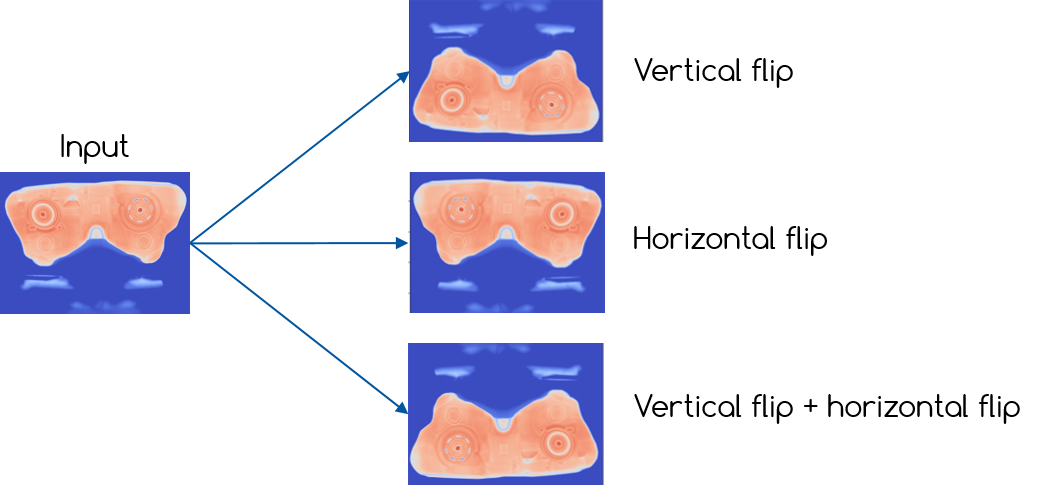
\includegraphics[scale=0.8]{images/chapter_4/data_augmentation.png}
\caption{Image augmentation}
\label{fig:image_augmentation}
\end{figure}

As image colour is temperature related, any augmentation techniques that alter the colour space risk corrupting the input data.
While the lack of a large volume of input data can be handled by transfer learning and data augmentation, the lack of labelled data in the training dataset can be a little more challenging. In fact, since the full thickness map of the part is not available, we cannot train the model in the traditional pixel-wise loss between the ground truth map and its reconstruction computed by the network. The computed loss is then back-propagated in the network to adjust the learnable parameters of the architecture. In our particular case, the full thickness ground truth of the part is not known, which means that we cannot compute the pixel-wise loss everywhere. However, it is possible to train the network by computing the pixel-wise loss between the map and the reconstruction for the pixels whose thickness is known.

\section{Experimental Validation} \label{Experimental Validation}

This section presents the results from a real-world implementation in an industrial setting. First, the empirical context is described as well as the data processing and the training pipeline. Finally, we provide the results of this first experimentation.

\subsection{Data collection}

To evaluate the performance of the proposed data-driven model-based quality control, a data acquisition campaign in an industrial environment has been organised. In order to train our models to learn to infer the thickness, given the cooling profile, we need two different types of data: the temperature of the part surface and the thickness measurement of the corresponding part. The temperature data  has been acquired with an industrial thermal camera OPTRIS PI 640 with a good resolution (640$\times$480), previously calibrated to correctly measure the temperature of the plastic material. Unlike traditional colour images, which are commonly represented using a 3-channel matrix (\textit{RGB}) with 256 different integer values, thermal images collected through the OPTRIS 640 PI are 1-channel matrices where each pixel takes a continuous value corresponding to a temperature in degrees Celsius. Unlike other temperature measuring instruments, the thermal camera has the advantage to evaluate, in a single shot, the temperature of the whole visible surface. Several consecutive shots of the same part make it possible to follow the evolution of the temperature over time (Figure \ref{fig:thermal_video}). 

Before moving forward to the description of the empirical context, a clarification is needed. Previously, we said that thermal images are 1-channel matrices where each pixel takes a continuous value corresponding to a temperature in degree Celsius. Because computers interprets as images only matrix (or 3D tensors) composed of unsigned integers ranging from 0 to 255, to display a thermal image is necessary to map the continuous temperatures values to the 0-255 range. In others words, a \textit{colormap} needs to be applied to the raw images in order to display it. In Figure \ref{fig:thermal_video}, as well as for others images of the current chapter, raw thermal frames are transformed in RGB images using a colormap which map low temperature value to blue colours and high temperature value to red colours. In order to have comparable colours among the different frames the colormap is computed on values ranging from 40°C (dark blue) and 135°C (bright red).  

\begin{figure}
\centering
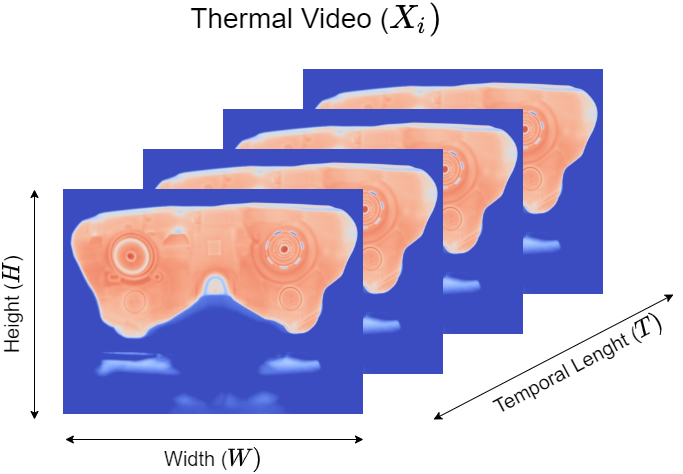
\includegraphics[scale=0.55]{images/chapter_4/Thermal_video.png}
\caption{Thermal video $X_i$}
\label{fig:thermal_video}
\end{figure}

Of course, measuring the temperature of the entire surface of the part would require several cameras. In the presented experiment, we limit the temperature acquisition to half of the whole surface. The thickness measurement has been carried out on key points through the use of an ultrasonic measurement instrument routinely used for sampling control. The thickness of the part selected for our experimentation have typical values ranging between 3 and 10 millimetres. In order to gather comparable data, the image acquisition of each part produced needs to be synchronised with the blowing process in order to synchronise the  acquisition of images on the same relative time. Repeatable mechanical movements of the machine have been used to “trigger” data acquisition. The trigger starts a one minute countdown after which the acquisition of thermal images begins. This time is mandatory to give the machine the time to unload the part and the machine operator time to place the part in the measuring area. For our experimental measurement campaign, we collected thermal videos on 50 different parts. For each part we recorded 120 consecutive thermal images equally spaced with a one second interval between images, for a total of two minutes of data acquisition. For each thermal video, and therefore for each part, we measured 20 critical thickness points evenly distributed on the tank surface (Figure \ref{fig:critical_points}).

\begin{figure}
\centering
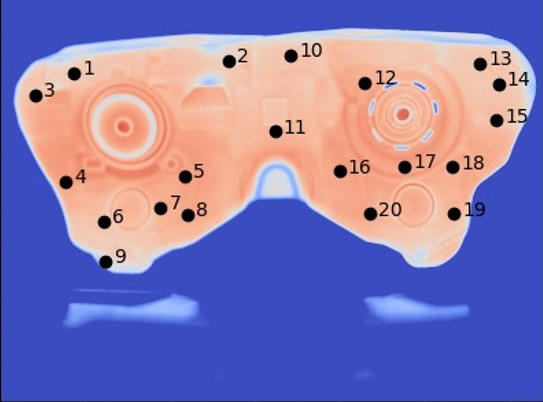
\includegraphics[scale=1]{images/chapter_4/critical_points.jpg}
\caption{Critical points distribution on the tank surface}
\label{fig:critical_points}
\end{figure}

\subsection{Data processing}

Once the data has been collected, some processing operations are needed to prepare the data for training. In particular, we need to associate the 20 key points whose thickness is measured to their corresponding pixel coordinates on the thermal video. This was done manually, each measured point of the part is identified on a thermal image by its $(\xi_{k}, \zeta_{k})$ pixel coordinate. Hopefully, since the position of the part does not change during the image acquisition, it is sufficient to find the pixel coordinates for one frame per sequence. 

Although the part does not move during the acquisition, each part is not precisely positioned with respect to the field of view of the thermal camera. The  $(\xi_{k}, \zeta_{k})$ coordinates on different thermal videos may therefore refer to different surface areas of the part. In order to align pixel coordinates along parts, a transformation is applied, to each frame, to project the part onto a reference position. Before describing the transformation in more detail, we present the \textit{pinhole camera model}. 

\paragraph{The pinhole camera model}
The pinhole camera model describes the mathematical relationship between the coordinates of a point in a three-dimensional space and its projection onto a two-dimensional pixel coordinate system. This mathematical relationship depends on the extrinsic and intrinsic parameters of the camera. The extrinsic parameters refer to the rotation matrix and translation vector of the camera coordinate system with regard to the world coordinate system.
Given a point $(x, y, z, 1)^{T}$ in the world coordinate system, we can form its pixel coordinates $(u, v, 1)^{T}$ as follows:
\begin{equation} \label{pinhole}
    \begin{bmatrix} u\\ v\\ 1 \end{bmatrix} = \begin{bmatrix}
        f_x & 0   & c_x\\ 
        0   & f_y & c_y \\ 
        0   & 0   & 1 
        \end{bmatrix}
        \begin{bmatrix}
        r_{11}& r_{12} & r_{13} & t_{x} \\ 
        r_{21}& r_{22} & r_{23} & t_{y} \\
        r_{31}& r_{32} & r_{33} & t_{z}
        \end{bmatrix}
        \begin{bmatrix} x\\ y\\ z \\ 1 \end{bmatrix}
        \enspace,
\end{equation}
That is:
\begin{equation}
    \begin{bmatrix} u\\ v\\ 1 \end{bmatrix} = K[R|T]
    \begin{bmatrix} x\\ y\\ z \\ 1 \end{bmatrix}
        \enspace,
\end{equation}

where:
\begin{itemize}
    \item $K$ is the 3 $\times$ 3 intrinsic camera matrix.
    \item $f$ is the focal length.
    \item $(c_x,c_y)$ are the coordinates of the principal point at the center of the image plane.
    \item $R$ is the 3 $\times$ 3 rotation matrix.
    \item $T$ is the translation vector.
    
\end{itemize}

Given this  mathematical description, a homography $H$ can be defined as a transformation matrix that maps points from one plane to another. It can be derived by the equation \ref{pinhole}:

\begin{equation}
    \begin{bmatrix} u\\ v\\ 1 \end{bmatrix} = \begin{bmatrix}
        f_x & 0   & c_x\\ 
        0   & f_y & c_y \\ 
        0   & 0   & 1 
        \end{bmatrix}
        \begin{bmatrix}
        r_{11}& r_{12} & r_{13} & t_{x} \\ 
        r_{21}& r_{22} & r_{23} & t_{y} \\
        r_{31}& r_{32} & r_{33} & t_{z}
        \end{bmatrix}
        \begin{bmatrix} u'\\ v'\\ 0 \\ 1 \end{bmatrix}
\end{equation}

\begin{equation}
    \begin{bmatrix} u\\ v\\ 1 \end{bmatrix} = \begin{bmatrix}
        f_x & 0   & c_x\\ 
        0   & f_y & c_y \\ 
        0   & 0   & 1 
        \end{bmatrix}
        \begin{bmatrix}
        r_{11}& r_{12} & t_{x} \\ 
        r_{21}& r_{22} & t_{y} \\
        r_{31}& r_{32} & t_{z}
        \end{bmatrix}
        \begin{bmatrix} u'\\ v'\\ 1 \end{bmatrix}
\end{equation}

\begin{equation}
    \begin{bmatrix} u\\ v\\ 1 \end{bmatrix} = 
        \begin{bmatrix}
        h_{11}& h_{12} & h_{13} \\ 
        h_{21}& h_{22} & h_{23} \\
        h_{31}& h_{32} & h_{33}
        \end{bmatrix}
        \begin{bmatrix} u'\\ v'\\ 1 \end{bmatrix}
\end{equation}

\begin{equation} \label{projection}
P=HP'
\end{equation}

where:

\begin{itemize}
    \item $P$ and $P'$ are two points on different planes.
    \item $H$ is a 3 $\times$ 3 matrix composed by intrinsic and extrinsic parameters that relate the two planes together.
\end{itemize}


The mathematical framework presented above can be applied to project all the thermal frames composing the 50 thermal video collected over a reference image. By estimating the homography between the two planes, that of the reference image and that of the image to be projected, each point $P$ of the input image can be projected to the reference image. 

The first frame of each thermal video sequence is used to estimate the homography matrix, through the use of the ORB (Oriented FAST and Rotated BRIEF) algorithm \citep{rublee2011orb}. In a nutshell, ORB is a feature matching algorithm that allows to automatically find some key points in an image. The ORB algorithm takes as inputs two images, a reference and the one we want to project on this reference, and features that can be matched in the two images are used to estimate the homography matrix. Once the homography is computed, it is applied to map all the pixels of the second image to the pixel of the reference image. The same transformation can then be applied to all the frames in the video sequence, provided that both the camera and the tank are motionless. 
%
Then, depending on the used method, extra processing is needed to prepare data for training.

\subsubsection{Parametric temporal approach}
The parametric temporal approach makes use of the temperature time series extracted from the thermal video sequences to infer the corresponding thickness. Given the coordinates $(\xi_{k}, \zeta_{k})$ of the 20 critical thickness values, it is simple to retrieve the temperature time series by simply collecting the temperature of the coordinate for each sequential frame of the thermal video. By extracting all temperature time series for each critical point of the 50 parts considered, we can build a new time series dataset composed of 1000 (50 x 20) time series and the corresponding thickness values. The time series are then approximated by their parametric expansion. As explained in Section \ref{Parametric Temporal approach}, three different parametric functions have been identified as good candidates for approximating the pixel-wise temperature surface decay. In order to identify the parametric expansion that best fits the input time series, each expansion was applied to the time-series of the training set. The root mean square error (RMSE) of the overall reconstruction is used to select the best expansion. 

Table \ref{tab:curve_fitting_error} shows the average RMSE reconstruction for the three parametric expansions considered. The polynomial expansion minimises the reconstruction error and is thus used to summarise the raw time series.  
For each time series, the three parameters defining the second-order polynomial approximation constitute the predictor of the machine learning model.

\begin{table}
\centering
\caption{Curve fitting reconstruction error}
\begin{tabular}{ll}
\toprule
Parametric function    & RMSE (train) \\ 
\midrule

Power Law              & 0.29         \\ 
Logarithmic            & 0.27         \\ 
Polynomial (2nd degree) & 0.03         \\ 
\bottomrule
\end{tabular}
\label{tab:curve_fitting_error}
\end{table}


\subsubsection{Flexible temporal approach}

As for the parametric temporal approach, the flexible temporal approach makes use of the temperature time series extracted from the thermal video sequences to infer the corresponding thickness. Given the coordinates $(\xi_{k}, \zeta_{k})$ of the 20 critical thickness values, it is simple to retrieve the temperature time series by simply collecting the temperature of the coordinate for each sequential frame of the thermal video. Unlike the previous approach, no extra data processing is required because the raw time series constitute the input data of the RNN model. 

\subsubsection{Spatio-Temporal approach}
Compared to the previous approaches, the spatio-temporal approach does not require to rearrange the input thermal video in another format, but some processing operations are still needed to allow the usage of a pre-trained spatial encoder. In order to be consistent with the data of the \textit{ImageNet} dataset \citep{deng2009imagenet} that was used  to pre-train the network, each thermal frame is converted to a 3-channel RGB image. The maximum and minimum temperatures among all frames are retrieved and the same colormap is applied on all thermal frames of each video sequence. The colormap is the one applied to visualise the thermal frames in the current Chapter. All values are then rescaled in $[0, 1]$ and then normalised using the default mean and standard deviation value of the \textit{ImageNet} dataset.

\subsection{Training}

In this section our training pipeline is presented. For each approach, the data was divided into three sets: the training set (data from 38 parts), the validation set (data from 8 parts) and the test set (data from 5 parts). The training is used to fit the models, the validation set is used to select the model hyper-parameters and the test set is used to evaluate the ability of the model to generalise on new data. For each proposed approach, a Bayesian optimization of hyper-parameters with the \textit{Tree-structured Parzen Estimator} (TPE) \citep{bergstra2011algorithms} algorithm was used to select the hyper-parameters that minimise the \textit{Mean Squared Error} (MSE) on the validation set.

\subsubsection{Parametric temporal approach}

As explained previously, a second-degree polynomial is fitted over the time series to compress the input data into a few features corresponding to the coefficients of the polynomial expansion of the thermal signal. Three machine learning algorithms were compared to model the relationship between the polynomial coefficients and the corresponding thickness values: \textit{Lasso} (linear) regression, \textit{random forest} and \textit{Support Vector Machine} (linear or kernelised) regression. 
The exhaustive list of model hyper-parameters and their search space is summarised in Table \ref{tab:Parametric Temporal_search_space}.

\begin{table}
\centering
\caption{Hyper-parameter search space for the parametric temporal models}
\label{tab:Parametric Temporal_search_space}
\begin{tabular}{lll} 
\toprule
\textbf{Model}                            & \textbf{Hyper-parameter} & \textbf{Search space}                          \\ 
\midrule
Lasso                                     & $\lambda$                & LogSpace($10^{-5}$, 1)                          \\ 
\midrule
SVM  & Kernel                   & \{Linear, Polynomial, RBF\}  \\ 
\cline{2-3}
                                          & $C$                        & LogSpace($10^{-6}$, 1)                          \\ 
\cline{2-3}
                                          & Polynomial degree (Polynomial) & [2, 4] \\
\cline{2-3}
                                          & $\gamma$ (\{Polynomial, RBF\}) & LogSpace($10^{-3}$, $10^{3}$) \\
                                          
\midrule
\multirow{3}{*}{Random Forest}  & Number of predictors     & [50, 500]                       \\ 
\cline{2-3}
                                          & Maximum tree depth       & [4, 50]                           \\ 
\cline{2-3}
                                          & Minimum samples leaf     & [1,60]                           \\
\bottomrule
\end{tabular}
\end{table}

\subsubsection{Flexible temporal approach}
We compared the performances of three RNN-based models: a vanilla RNN, an LSTM and finally a GRU network. The number of hidden units of each computational cell, as well as the number of stacked layers are hyper-parameters that are optimised. A comprehensive summary of the search space for the hyper-parameters is available in Table \ref{tab:rnn_search_space}. 

\begin{table}
    \centering
    \caption{Hyper-parameter search space for the flexible temporal models}
    \begin{tabular}{ll}
    \toprule
    \textbf{Hyper-parameter} & \textbf{Search space} \\ 
    \midrule
    RNN Cell type & \{RNN, LSTM, GRU\} \\
    N° hidden unit & \{8, 16, 32\} \\
    N° stacked layers & \{1, 2\} \\
    \bottomrule
    \end{tabular}
    \label{tab:rnn_search_space}
\end{table}
Each model has been trained to minimise the mean squared error metric using the  \textit{Adam} optimiser~\citep{kingma2014adam} with $\beta_{1} = 0.9$, $\beta_{2} = 0.98$ and $\epsilon = 10^{-9}$ (default values) and a learning rate sampled by the TPE algorithm on a logarithmic scale,  from $10^{-7}$ to $10^{-2}$. 

\subsubsection{Spatio-Temporal approach}
As for the previous approach, we compared different model configurations on two pre-trained networks: a ResNet18 (18 layers) and a ResNet34 (34 layers). Deeper architectures exist, but we made the choice to limit the search space to the two smaller ResNet architectures because of the limited number of samples in our training set. Deeper architectures would allow to extract richer data representations, but at the expense of more parameters and increased computation time. We believe that ResNet18 and ResNet34 are powerful enough to produce a relevant representation of thermal images. Another hyper-parameter of the presented architecture is the number of encoder/decoder blocks. As stated in Section \ref{Residual Networks}, all ResNet architectures, independently on their depths, have 5 main building blocks. Actually, it is possible to slightly change the architecture in order to stop the encoding computation before the last block. This allows to reduce the complexity of the architecture and thus prevent possible over-fitting problems. For instance, we could take into account only the first 3 convolutional building blocks of the ResNet in such a way that the output of the third convolutional building block would be the spatial feature map and the output of the first and second blocks would be the intermediate encoded features. Since the encoder and decoder are symmetrical, reducing the number of encoder blocks also implies a reduction in the number of decoder blocks.

\begin{table}[h!]
    \centering
    \caption{Hyper-parameter search space for the spatio-temporal models}
    \begin{tabular}{ll}
    \toprule
    \textbf{Hyper-parameter} & \textbf{Search space} \\ 
    \midrule
    Encoder & \{ResNet18, ResNet34\} \\
    N° of blocks  & \{3, 4, 5\} \\
    \bottomrule
    \end{tabular}
    \label{tab:spatial_temporal_search_space}
\end{table}

As for the flexible temporal approach, each model configuration has been trained to minimise the MSE metric using \textit{Adam} optimiser with $\beta_{1} = 0.9$, $\beta_{2} = 0.98$ and $\epsilon = 10^{-9}$ and a learning rate sampled by the TPE algorithm on a logarithmic scale from $10^{-10}$ to $10^{-2}$. 

\subsection{Results}

In this section the results obtained with the three approaches are presented and compared. Performances are measured using the Root Mean Squared Error (RMSE), which has the benefit of penalising large errors and whose value is easy to interpret because it has the same unit as the dependent variable: all the scores presented below represent the average thickness reconstruction error in millimetres.

For the parametric temporal approach, random forest performs better in both fit on the training set and generalisation on the test set (Table \ref{tab:Parametric Temporal_model_results}).
%
\begin{table}[h]
    \centering
    \caption{RMSE for the parametric temporal models}
    \begin{tabular}{llll}
     \toprule
    \textbf{Model} & \textbf{Train}  & \textbf{Validation}  & \textbf{Test}  \\
    \midrule
    Lasso & {0.95} & {0.91} & {0.89} \\
    Support Vector Regressor & {0.80} & {0.73} & {0.76} \\
    Random Forest Regressor & {0.19} & {0.54} & {0.48} \\
    \bottomrule
    \end{tabular}
    \label{tab:Parametric Temporal_model_results}
\end{table}
%
The error is about 0.5 mm, which is not accurate enough from the industrial point of view. However, this first experiment allowed us to demonstrate that there is a relationship between the temperature evolution of a zone of the part and the corresponding thickness, as assumed in  Section \ref{Motivation}.

\begin{figure}
\centering
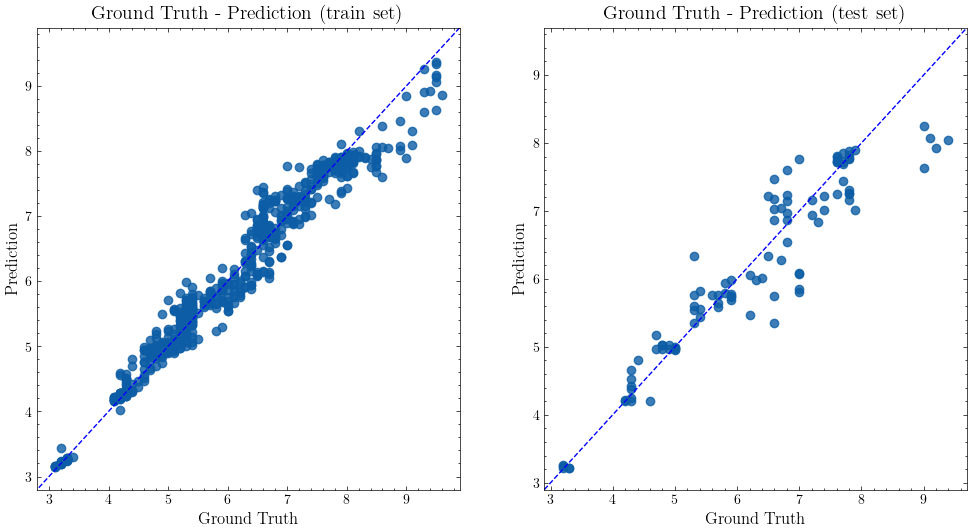
\includegraphics[scale=0.48]{images/chapter_4/temporal_scatter.png}
\caption{Prediction \textit{versus} ground truth scatter plots in train (left) and test (right) for the parametric temporal approach based on random forest regression}
\label{fig:gt_prediction_functional}
\end{figure}

Figure \ref{fig:gt_prediction_functional} shows the scatter plots of the predicted thickness and ground-truth thickness for the training and test sets. The plots confirm the ability of the model to distinguish between large and small thicknesses. Moreover, they show that the model is more accurate for thin points (close to 3 mm), which is positive because the thinnest points are also the most critical for the part to meet the customer's specifications.

Among all flexible temporal trained model, the configuration that minimises the validation error is a GRU model with 8 hidden units per cell and one layer. The results obtained are summarised in Table \ref{tab:temporal_model_results}.
%
\begin{table}
    \centering
    \caption{RMSE for the flexible temporal models}
    \begin{tabular}{llll}
    \toprule
    \textbf{Model} & \textbf{Train}  & \textbf{Validation}  & \textbf{Test}  \\
    \midrule
    RNN & {0.55} & {0.58} & {0.58} \\
    LSTM & {0.54} & {0.57} & {0.56} \\
    GRU & {0.54} & {0.56} & {0.54} \\
    
    \bottomrule
    \end{tabular}
    \label{tab:temporal_model_results}
\end{table}
%
These results are similar to those obtained with random forest, but random forest has a slightly lower error than GRU. Moreover, the computation time needed to train the random forest is significantly lower and it does not rely on dedicated hardware (GPU). The parametric temporal approach therefore seems preferable in all respects. This is confirmed in Figure~\ref{fig:gt_prediction_temporal}, where the parametric temporal approach outperforms the flexible temporal approach over all thickness ranges.
\begin{figure}
\centering
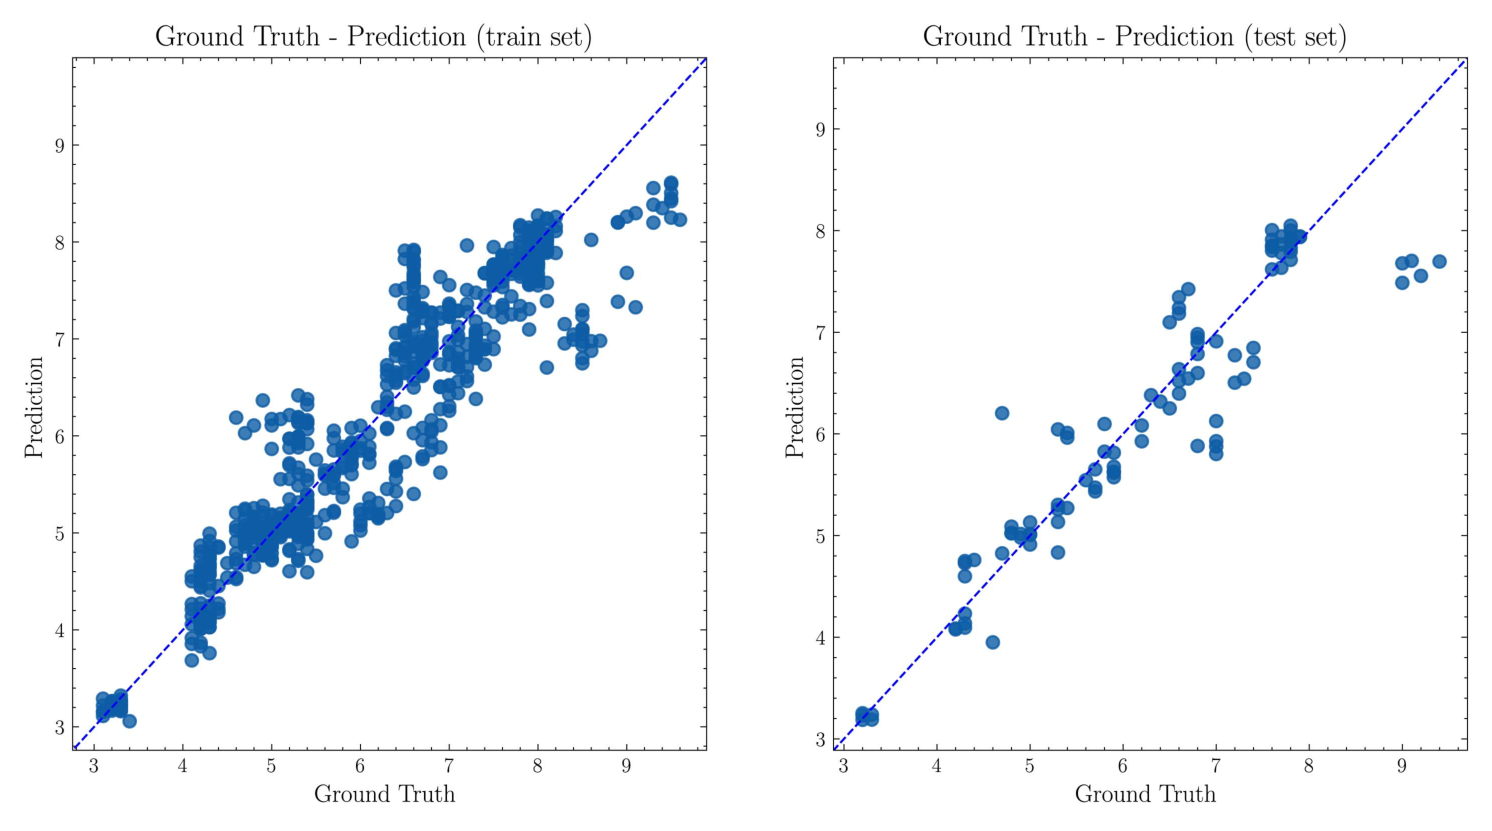
\includegraphics[scale=0.48]{images/chapter_4/gt_temporal.eps}
\caption{Prediction \textit{versus} ground truth scatter plots in train (left) and test (right) for the flexible temporal approach based on GRU}
\label{fig:gt_prediction_temporal}
\end{figure}

The third approach (Table \ref{tab:spatial_temporal_model_results}) completely outperforms the previous ones. The best results are obtained using a pre-trained ResNet34 encoder with 5 encoder-decoder blocks, which achieves an RMSE of 0.16 mm on the test set, which is about one-third of the error of the previous approaches. A precision of 0.2mm is considered extremely interesting in our industrial context. 
\begin{table}
    \centering
    \caption{RMSE for the spatio-Temporal model}
    \begin{tabular}{llll}
    \toprule
    \textbf{Model} & \textbf{Train}  & \textbf{Validation}  & \textbf{Test}  \\
    \midrule
    ResNet34-5 blocks & \textbf{0.14} & \textbf{0.18} & \textbf{0.16} \\
    \bottomrule
    \end{tabular}
    \label{tab:spatial_temporal_model_results}
\end{table}
Figure~\ref{fig:gt_prediction_spatial_temporal} shows that the greatest benefits over the parametric temporal approach are at higher thicknesses, but the improvement is already visible at only 4 mm.

\begin{figure}
\centering
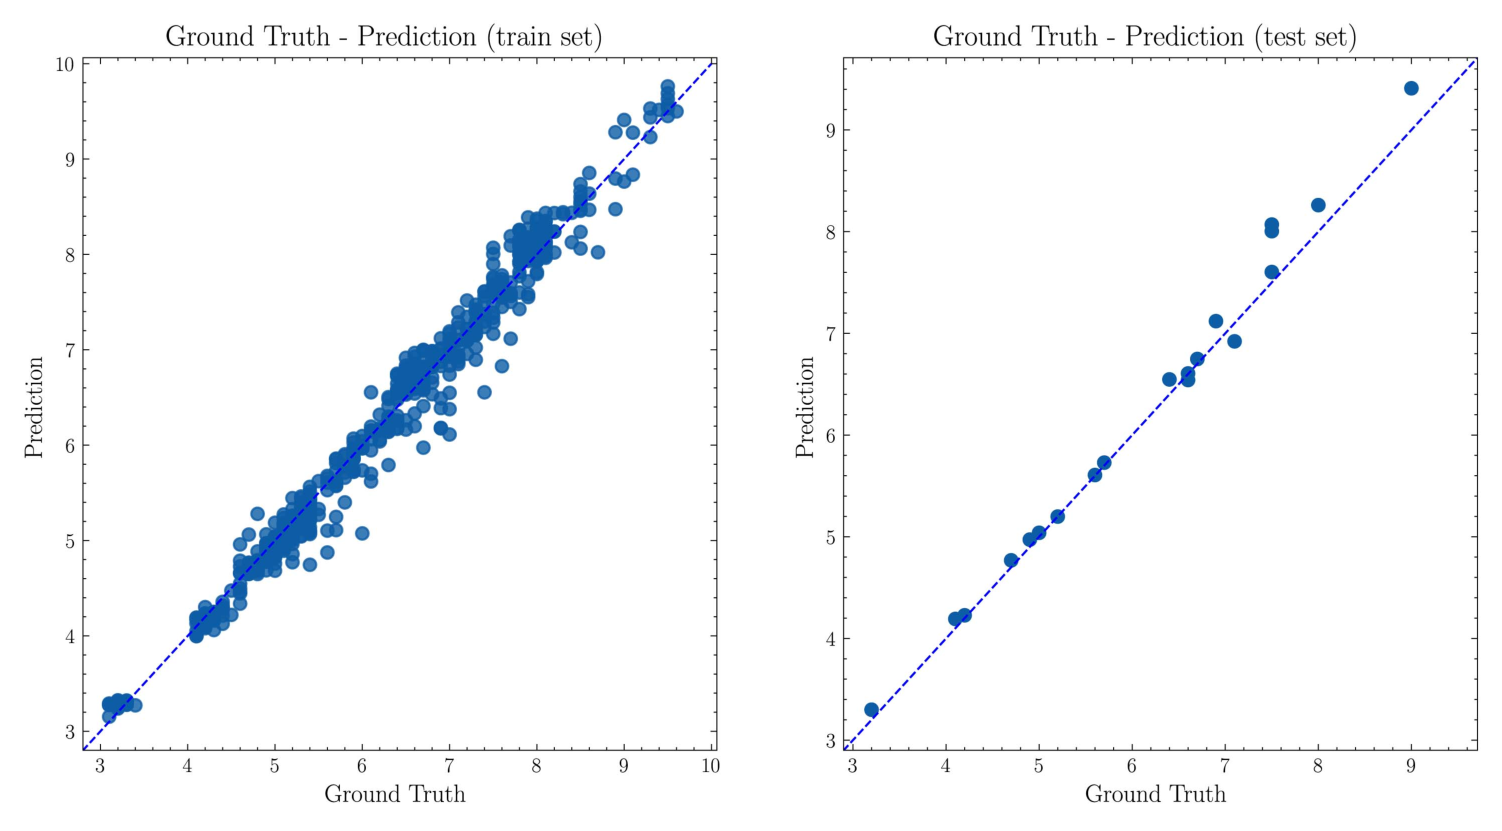
\includegraphics[scale=0.48]{images/chapter_4/gt_spatial_temporal.eps}
\caption{Prediction \textit{versus} ground truth scatter plots in train (left) and test (right) for the spatio-temporal approach based on ResNet34}
\label{fig:gt_prediction_spatial_temporal}
\end{figure}

\subsection{Model performance on unseen data point}

The results presented in the previous section show the ability of the spatio-temporal model to correctly estimate the thicknesses at the critical points of the part. The question is whether the model is able to generalise the relationship learned at a limited set of critical points to the entire surface of the part. The spatio-temporal architecture computes a thickness map for the entire surface of the tank. An example of the thickness map produced in this way is shown in Figure \ref{fig:thickness_mask_reconstruction} for a part in the test set. 
In this figure, the colour represents the predicted thickness, not the tank temperature.
The figure highlights the ability of the model to produce a thickness reconstruction beyond the critical points, but some areas, especially those close to the edge of the tank, are more difficult to predict. 
The prediction of thicknesses outside the critical points is unreliable.

\begin{figure}
\centering
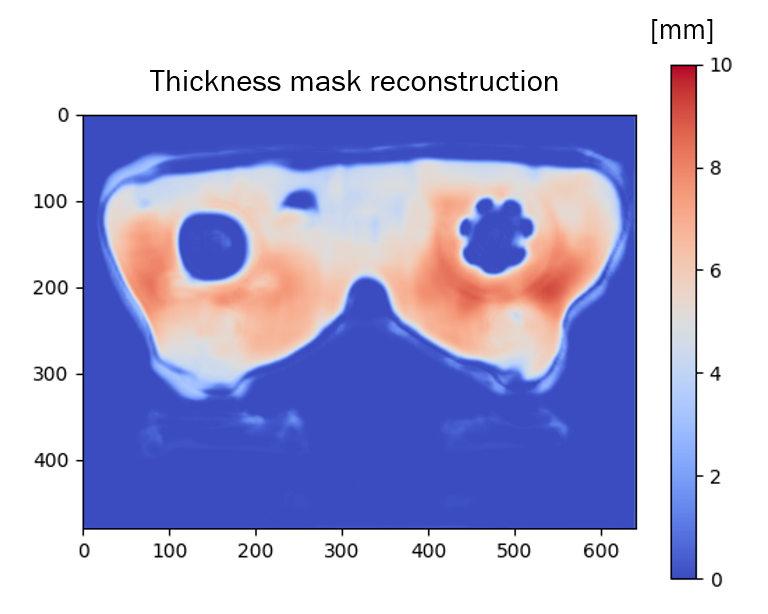
\includegraphics[scale=0.90]{images/chapter_4/mask_reconstruction.png}
\caption{Thickness mask reconstruction example}
\label{fig:thickness_mask_reconstruction}
\end{figure}

We modified the evaluation strategy to test accurately the accuracy of predictions outside of the measured critical points.
Since the entire thickness map is not available, we used only a subset of the 20 critical points to train the model, reserving the others to compute an out-of-critical-point prediction error. We removed 4 out of 20 critical points of the training set to adjust the model on the remaining points. The 4 points removed are then used to evaluate the ability of the model to predict the thickness outside critical points on test parts. This was repeated 20 times by randomly selecting the 4 removed points, to evaluate the results on a larger set, composed of $4\times20$ samples.
The results are presented in Figure \ref{fig:gt_prediction_unseen}, which shows a positive correlation between ground truth and prediction. 
%
\begin{figure}
\centering
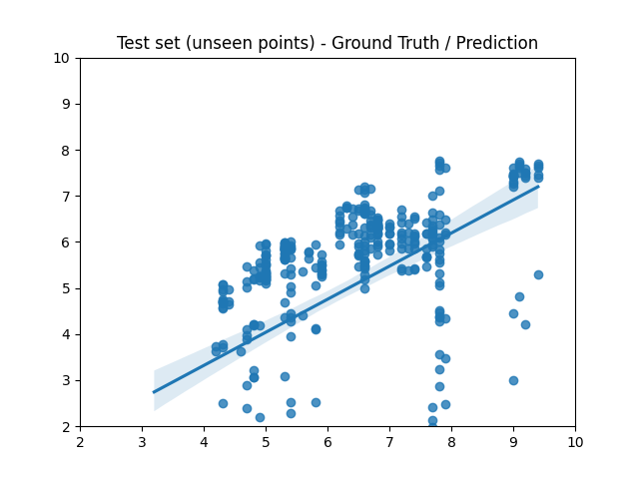
\includegraphics[scale=0.90]{images/chapter_4/unseen_point_scatter.png}
\caption{Prediction \textit{versus} ground truth scatter plot for the spatio-temporal approach based on ResNet34 on critical points not seen in training}
\label{fig:gt_prediction_unseen}
\end{figure}
%
However, the prediction of the thickness of unseen points is nowhere near as good as the prediction on these critical points, and our approach does improve on the manual inspection in this respect: our model is reliable on the critical points usually measured but fails to predict the thickness of the entire part. In Chapter \ref{Contributions and perspectives} we will present some of the research perspectives we are working on to improve the ability of the model to correctly predict the thickness of the full visible surface. 

% Perspectives 

\section{Conclusion}

Traditional quality control methods for measuring blow-moulded part thickness involves time-consuming operations that cannot be applied online for a 100\% quality inspection on all parts. This chapter proposes a new data-driven approach for measuring in real-time the part thickness by leveraging the surface-temperature decay over time. Three different pipelines have been designed to model the relationship between the cooling behaviour of a part area, captured through the use of a thermal camera, and the corresponding thickness. The procedure was validated in a real-world manufacturing setting. These results have shown the ability of our method to provide accurate results in predicting thickness values of a set of critical points. Among the three pipelines presented above, the spatio-temporal approach is the one that achieve the best performance in reconstructing the thickness values of the test set data. Future research works aim to generalise predictions outside of the critical points, in order to reconstruct the full thickness map of the whole visible part surface. In Chapter \ref{Contributions and perspectives} we will provide more details about the research perspectives related to this topic. 

\subsection{Scientific Contribution}

Thermography for measuring thickness is not a new idea, however, to our knowledge, this is the first time that thermography has been proven to be effective at measuring the thickness of a part in an industrial environment. Certainly the first time it has been used to infer the thickness of a blow-moulded part. By leveraging the surface-decay temperature due to the part cooling at the room temperature, we can infer the thickness of a tank in a non-contact manner.

Compared to previous proposed approaches using thermography, which make use of physics-based approaches to compute thickness given the surface decay temperature, we have decided to leverage the ability of data-drive methods to discover hidden patterns within data. The idea of using a data-driven approach is dictated by the following two motivations:

\begin{itemize}
    \item The tank is composed of multiple layers of different plastic material which complicates physical modelling. The physic model should take into consideration the different physical properties of each layer constituting the thickness of the fuel tank.
    \item The thermal inertia of the material, which causes an initial rise in temperature in the first few seconds after the tank has been blow-moulded, have to be taken into account. In our opinion, it is simpler to model this phenomenon through a data-driven approach. 
\end{itemize}

Transfer learning has been proven to be effective in a context where the number of data was very limited. Although the proposed method was validated in a single case study, we claim it should generalise to other industrial contexts. The presented empirical setting was designed to respond to a specific need of a manufacturer, but we think it should apply to others manufacturer dealing with blow-moulding and others manufacturing process involving plastic processing. Whenever it is possible to observe a different cooling behaviour between different areas of the part surface, our approach may be potentially applied.


\subsection{Industrial Contribution}

From the industrial point of view, this chapter introduces a new idea of quality control. The traditional Acceptance Sampling approach, used in the industrial context studied, may be enhanced by introducing data-driven model quality control. In this chapter we have shown that by adding extra sensors, or cameras, it could be possible to infer the quality of the part and therefore provide a quality status in real-time without any time-consuming or destructive measurement. This provides to the manufacturing company a dual benefit:
%
\begin{itemize}
    \item It ensures a quality control on all parts produced which enable for a fast reaction to quality non-conformities. In fact, by ``virtually'' measuring each part, we are able to eventually discard parts for which the model has provided a ``Not-OK'' result, or request the quality team to carry out more in-depth tests. Model-based quality measurement may be effectively used to detect those parts that turn out to be, from a statistical point of view, outliers. In this way, instead of randomly sampling the parts to be measured by the quality operators, the model is able to suggest the parts that seem to be interesting. By discarding all non-compliant parts, this approach indirectly reduces product recalls and thus the whole series of requests to return, exchange or replace a product that has been found to be defective, and which could impair performance, harm consumers or cause legal problems for producers.
    \item Such an approach could be applied to reduce the real quality controls which destroy the parts or makes them unusable. In such a case, not only the data driven model-based control would be able to provide a thorough quality control, but it would also be able to reduce the scraps which account for an overall better production performance. Of course, real part measurements cannot be completely replaced by model-based measurements. In fact, real measurements are the primary data source for training the data-driven model. 
\end{itemize}
%
As regarding the proposed approach to infer the thickness, results are considered accurate enough to move towards the industrialisation of the proposed system. In order to industrialise the proposed system, we should be able to take into account extra information such us the temperature of the environment where the machine is located, as well as the temperature of the moulds. In fact, the surface temperature of the blow-moulded part depends on the ability of the moulds to absorb the heat. If the heat absorption capacity changes, as a result of the change in temperature of the moulds coolant, the tank surface temperature will be different and the data-driven model accuracy would drop. In the same way, the plant temperature may influence a bit the cooling behaviour of the blow-moulded part. However, the impact of the temperature of the industrial environment on the surface temperature decay should be minimal due to the insulating properties of the plastic material (PEHD).  



